% Options for packages loaded elsewhere
\PassOptionsToPackage{unicode}{hyperref}
\PassOptionsToPackage{hyphens}{url}
%
\documentclass[
]{article}
\usepackage{amsmath,amssymb}
\usepackage{lmodern}
\usepackage{ifxetex,ifluatex}
\ifnum 0\ifxetex 1\fi\ifluatex 1\fi=0 % if pdftex
  \usepackage[T1]{fontenc}
  \usepackage[utf8]{inputenc}
  \usepackage{textcomp} % provide euro and other symbols
\else % if luatex or xetex
  \usepackage{unicode-math}
  \defaultfontfeatures{Scale=MatchLowercase}
  \defaultfontfeatures[\rmfamily]{Ligatures=TeX,Scale=1}
\fi
% Use upquote if available, for straight quotes in verbatim environments
\IfFileExists{upquote.sty}{\usepackage{upquote}}{}
\IfFileExists{microtype.sty}{% use microtype if available
  \usepackage[]{microtype}
  \UseMicrotypeSet[protrusion]{basicmath} % disable protrusion for tt fonts
}{}
\makeatletter
\@ifundefined{KOMAClassName}{% if non-KOMA class
  \IfFileExists{parskip.sty}{%
    \usepackage{parskip}
  }{% else
    \setlength{\parindent}{0pt}
    \setlength{\parskip}{6pt plus 2pt minus 1pt}}
}{% if KOMA class
  \KOMAoptions{parskip=half}}
\makeatother
\usepackage{xcolor}
\IfFileExists{xurl.sty}{\usepackage{xurl}}{} % add URL line breaks if available
\IfFileExists{bookmark.sty}{\usepackage{bookmark}}{\usepackage{hyperref}}
\hypersetup{
  pdftitle={Simple Linear Regression Lab},
  pdfauthor={Francesca Chiappetta},
  hidelinks,
  pdfcreator={LaTeX via pandoc}}
\urlstyle{same} % disable monospaced font for URLs
\usepackage[margin=1in]{geometry}
\usepackage{graphicx}
\makeatletter
\def\maxwidth{\ifdim\Gin@nat@width>\linewidth\linewidth\else\Gin@nat@width\fi}
\def\maxheight{\ifdim\Gin@nat@height>\textheight\textheight\else\Gin@nat@height\fi}
\makeatother
% Scale images if necessary, so that they will not overflow the page
% margins by default, and it is still possible to overwrite the defaults
% using explicit options in \includegraphics[width, height, ...]{}
\setkeys{Gin}{width=\maxwidth,height=\maxheight,keepaspectratio}
% Set default figure placement to htbp
\makeatletter
\def\fps@figure{htbp}
\makeatother
\setlength{\emergencystretch}{3em} % prevent overfull lines
\providecommand{\tightlist}{%
  \setlength{\itemsep}{0pt}\setlength{\parskip}{0pt}}
\setcounter{secnumdepth}{-\maxdimen} % remove section numbering
\usepackage{booktabs}
\usepackage{longtable}
\usepackage{array}
\usepackage{multirow}
\usepackage{wrapfig}
\usepackage{float}
\usepackage{colortbl}
\usepackage{pdflscape}
\usepackage{tabu}
\usepackage{threeparttable}
\usepackage{threeparttablex}
\usepackage[normalem]{ulem}
\usepackage{makecell}
\usepackage{xcolor}
\usepackage{amsmath}
\usepackage{caption}
\ifluatex
  \usepackage{selnolig}  % disable illegal ligatures
\fi

\title{Simple Linear Regression Lab}
\author{Francesca Chiappetta}
\date{9/29/2021}

\begin{document}
\maketitle

\#Summary Statistics \#\#1. Develop one table that displays the summary
statistics for both variables. Discuss the two variables in one
paragraph (total). Include a discussion of the correlation coefficient
between the two variables. (10 points)

\captionsetup[table]{labelformat=empty,skip=1pt}
\begin{longtable}{crrrrrrr}
\caption*{
{\large Summary Statistics of CO2 emissions and Urban Population Growth} \\ 
{\small CO2 in metric tons per capita, Urban Population Growth in annual percentage}
} \\ 
\toprule
Variable & Observations & Mean & Median & Minimum & Maximum & SD & Skewness \\ 
\midrule
CO2.Emissions & $162$ & $4.320745881$ & $2.613368118$ & $0.044485376$ & $34.16324263$ & $5.179291135$ & $2.488512130$ \\ 
Urban.Population.Growth & $162$ & $2.023192409$ & $1.837834954$ & $-1.123001709$ & $5.79180675$ & $1.588225525$ & $0.339320630$ \\ 
 \bottomrule
\end{longtable}
\begin{minipage}{\linewidth}
Data Source: World Bank\\ 
\end{minipage}

\#Histograms \#\#2. Develop histograms of the two variables that are
visually appealing and properly labelled

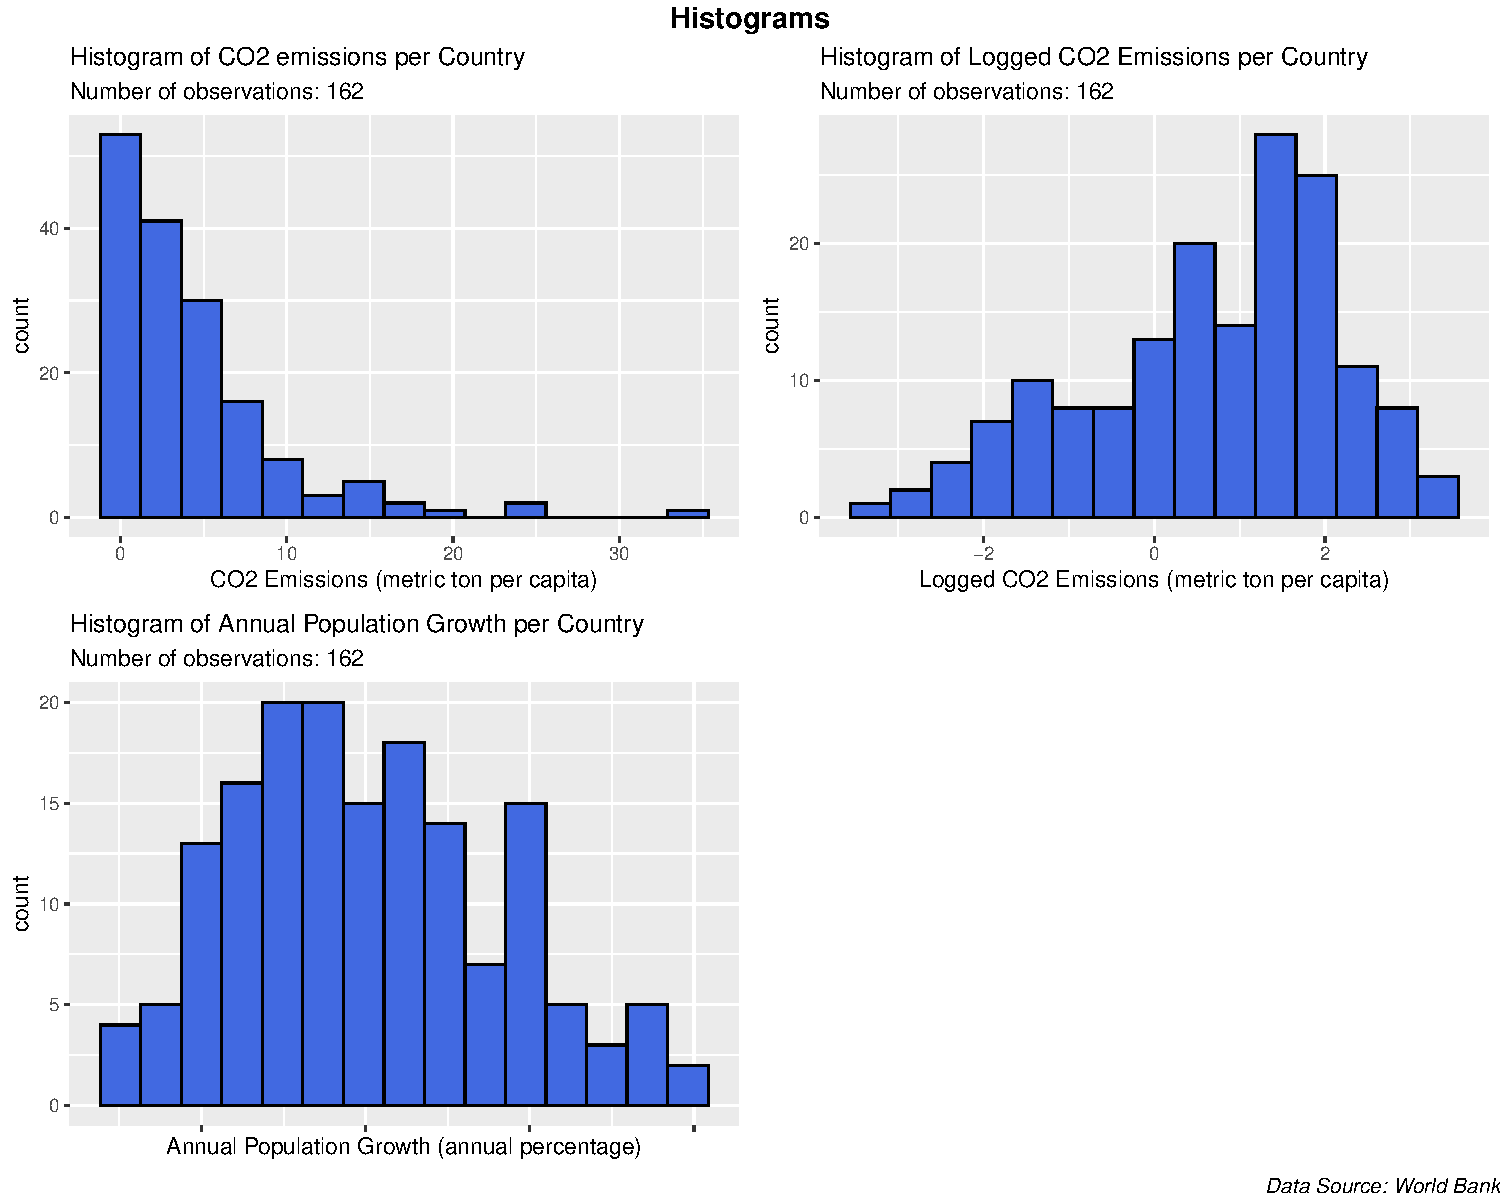
\includegraphics{LinearLab_files/figure-latex/unnamed-chunk-1-1.pdf}

\#Scatterplots \#\#3. Develop a scatterplot of the data. Explain clearly
which variable is the response and which is the explanatory. Discuss the
relationship between the two variables--is there a linear relationship
between the two variables? If there is not, consider a transformation of
one or both variables and rerun the scatterplot. (10 points) CO2:
response variable Pop growth: explanatory variable

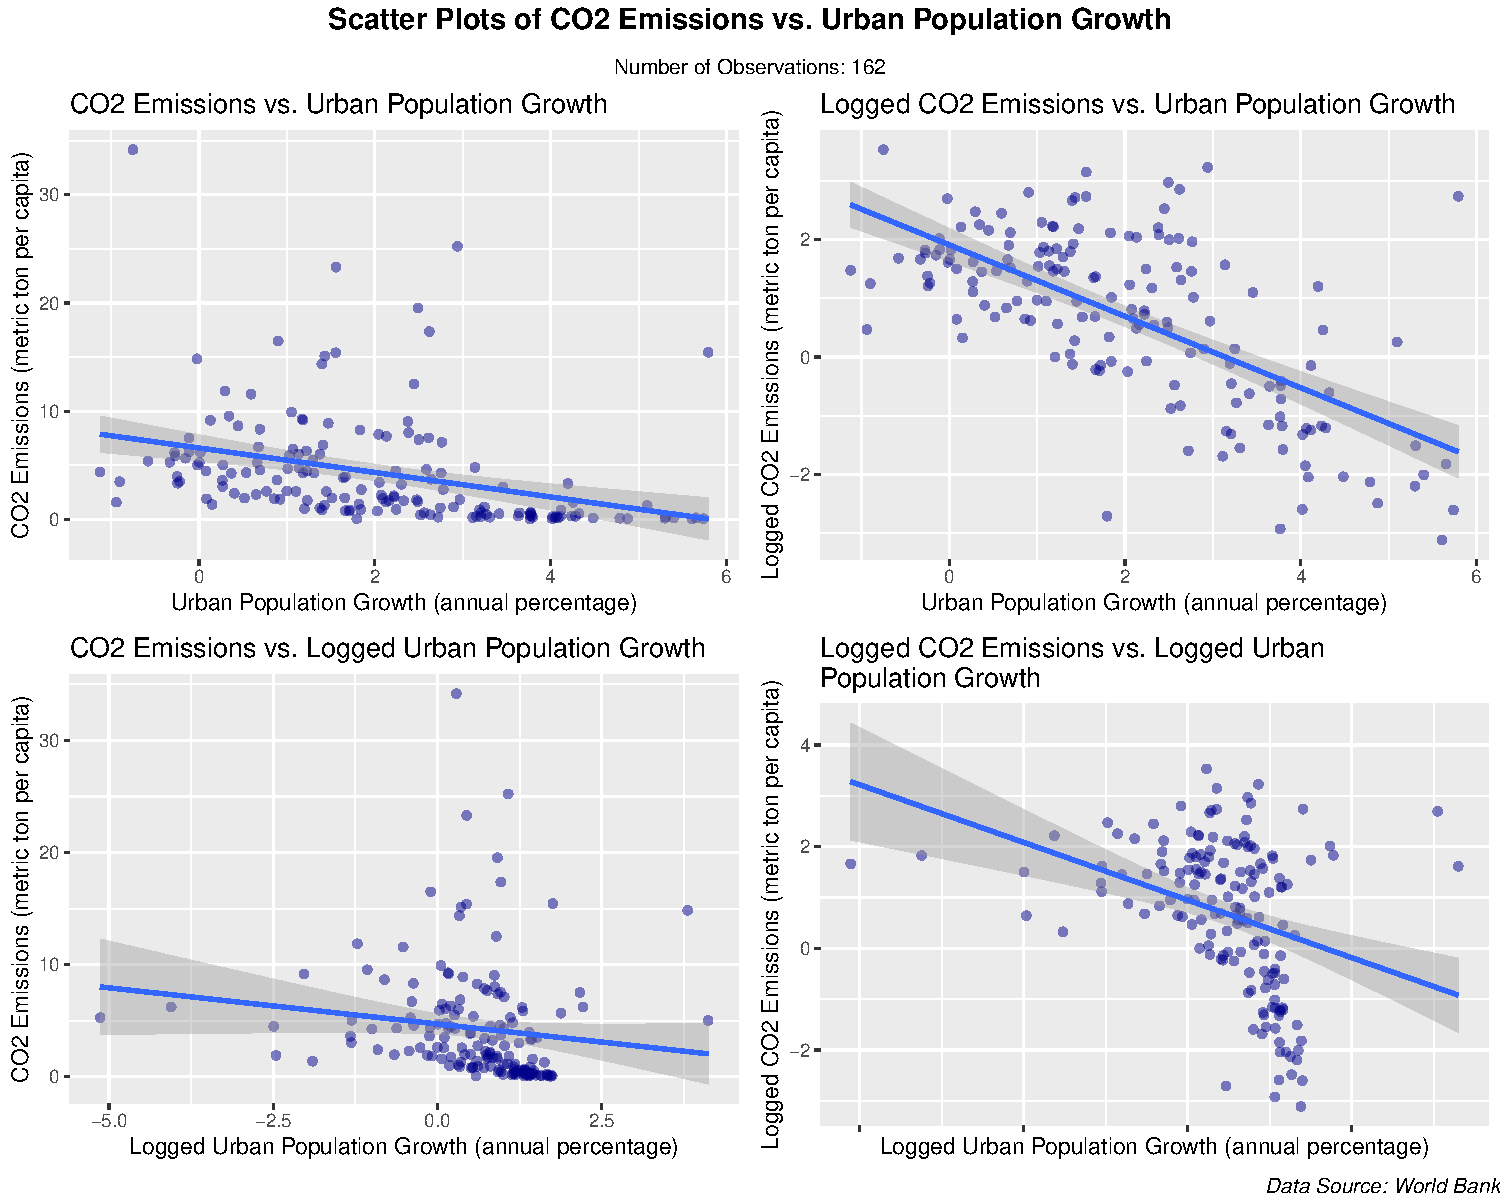
\includegraphics{LinearLab_files/figure-latex/scatterplots-1.pdf}

\#Linear Regression \#\# 4. Run a simple linear regression on the two
variables (or transformed variables based on \#3). Interpret the
coefficient estimate for the slope and its test of significance. (5
points). Discuss the R2 of the model (5 points)

Only the dependent/response variable is log-transformed. Exponentiate
the coefficient, subtract one from this number, and multiply by 100.
This gives the percent increase (or decrease) in the response for every
one-unit increase in the independent variable. Example: the coefficient
is 0.198. (exp(0.198) -- 1) * 100 = 21.9. For every one-unit increase in
the independent variable, our dependent variable increases by about
22\%.

y = -45.5551993 x + 1.90975

A one-unit increase in the explanatory variable (independent variable),
Urban Population Growth (annual percentage), decreases the response
variable (dependent variable), CO2 Emissions (metric tons per capita),
by 45.5551993\%.

The r-squared is how well the regression model fits the observed data
and generally, a higher r-squared indicates a better fit for the model.
The r-squared value of 0.43073 reveals that 43.072997 \% of the data fit
the regression model.

\#Residual vs.~Fitted Plots \#\# Run a residual vs fitted plot on the
regression you ran above. Discuss the underlying assumptions of an OLS
model and whether you think they are met in this context. (10 points).

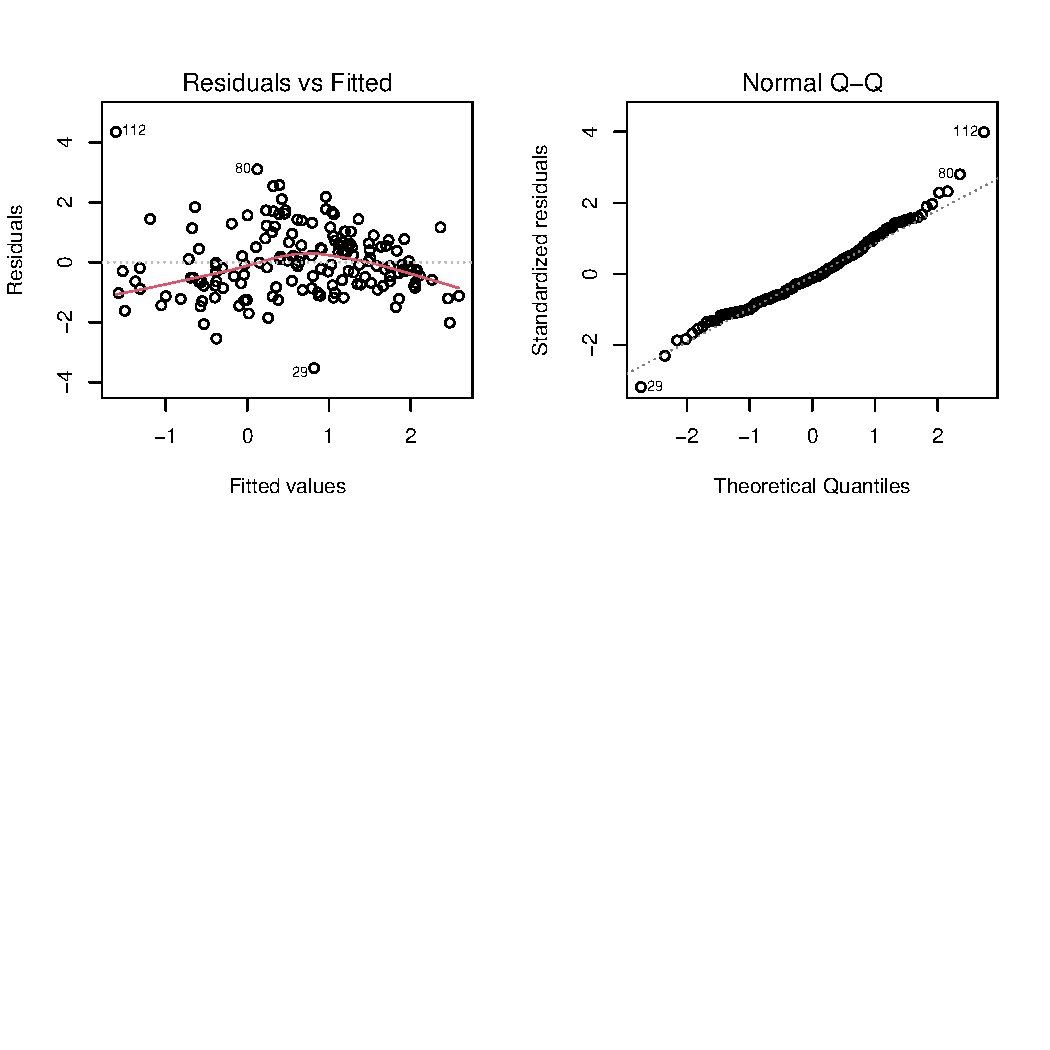
\includegraphics{LinearLab_files/figure-latex/res.vs.fit-1.pdf}

The first plot (residuals vs.~fitted values) is a simple scatterplot
between residuals and predicted values. It should look more or less
random and centered around 0.

The second plot (normal Q-Q) is a normal probability plot. It will give
a straight line if the errors are distributed normally.

\end{document}
